\section{Igrajući objekti}
Svaki objekt koji se može vidjeti u unity-u je \textbf{igrajući objekt} (\emph{eng. GameObject}). Kada se napravi bilo koj objekt on treba imati svoju poziciju unutar svijeta. Kako bi se mogla znati njegova pozicija koristimo komponente. Svaki objekt mora imati svoju transformaciju (\emph{eng. Transform}). U suštini igrajući objekti su samo kontenjeri koji sadrže komponente.
\subsection{Komponente}
Komponente su kao što je rečeno dijelovi igrajućih objekata. One daju funkcionalnost objektima, te omogućavaju krajnjim korisnicima da razlikuju igrajuće objekte. Neke važnije komponente koje su korištene za izradu igrice su:
\begin{itemize} 
	\item Transformacija
	\item Kruta tijela
	\item Sudarači
	\item Kolni sudarači 
\end{itemize}
\subsubsection{Transformacija}
Igrajući objekti moraju imati svoju \textbf{transformaciju}, inače se neće moći prikazati u svijetu. Transformacija definira širinu, poziciju i orijentaciju objekta. Svaka transformacija ima svoj pivot koji određuje centar, odnosno prema njemu se gledaju širina, pozicija i rotacija. Pivot se može gledati globalno ili lokalno. \par 
Globalno gledanje je pozicija pivota gledajući koordinate x,y,z svijeta. Lokalno gledanje pivota je relativna pozicija naspram pozicije objekta. Primjer transformacijog elementa (\emph{ Gizmo}) se može vidjeti na slici broj \ref{fig:kotaci}.
\newpage
\subsubsection{Kruta tijela}
Kruta tijela (\emph{eng. Rigid Body}) igrajućim objektima daju ponašanje kao u stvarnom svijetu. Objektima daju dodatne informacije kao na primjer masa, primjena sile za pomicanje objekata, hoće li vjetar utjecati na kretanje i tako dalje. Dodavajući kruta tijela može se isto definirati hoće li gravitacija utjecati na element. U igri je najvažnija informacija bila masa zbog bolje simulacija pravog automobila.
\subsubsection{Sudarači}
Sudarači (\emph{eng. Colliders}) su komponente koje omogućavaju igrajućim objektima fizičku koliziju. Oni se ne mogu vidjeti tokom igranja igre, a i nisu zbog toga napravljeni. Postoji više oblika sudarača (kvadar, sfera, kapsula, krug...) i svaki od njih se koristi za aproksimiranje mreže igrajućih objekata. Moguće je dodati sudarač tako da se savršeno slaže sa mrežom igrajućeg objekta, ali tada bi gubili na performansi. Jedan bolji način za bolju aproksimaciju je korištenje konveksnih (\emph{eng. Convex}) sudarača. Ovaj način dodaje mrežu sličnu modelu, ali izbaci neke dijelove. \par
Unity u svakom trenutku provjerava da li je sudarač imao koliziju sa nekim drugim igrajućim objektom koji isto ima svoj sudarač. Kada bi se oblik postavio da savršeno odgovara mreži igrajućeg objekta, tada bi trebalo obavljati previše računanja. U igri se koristi kvadratični sudarač za tijelo modela jer veoma dobro aproksimira automobil, a za kotače se koriste kolni sudarači.
\subsubsection{Kolni sudarači}
Unity ima predefinirane elemente za simulirati prave kotače prizemljenih vozila koje zovemo \textbf{kolne sudarače}. Prema dokumentaciji unity-a ovi sudarači se ne dodaju kao komponente, već trebaju biti komponente zasebnih igrajućih objekata. Znači za svaki kotač treba napraviti novi igrajući objekt, koji se zove prazni igrajući objekt (\emph{eng. Empty GameObject}). Doda se komponenta praznom objektu i cijeli objekt se pomakne tako da je centriran sa kotačima. \newpage \par
Najvažnije metode za vožnju su moment motora (\emph{eng. motor Torque}), moment kočnice (\emph{eng. brake Torque}), te kut okretanja (\emph{eng. steer angle}). Moment motora je sila koja djeluje na osovinu kotača izražena u Newton metrima. Predznak sile će odrediti smjer kretanja. Kut okretanja određuje za koliko će se okrenuti model prilikom skretanja, a moment kočnice određuje silu kočenja u Newton metrima. Primjer k\^oda za kretanje vozila se može vidjeti u ispisu \ref{fig:kotaci}

\begin{lstlisting}[caption={Skripta za kretanje vozila}, label=kretanjeVozila]
for(int i = 0; i < 4; i++)
    this.wheelsColliders[i].motorTorque = thrustTorque;
\end{lstlisting}

Jedan propust postoji kod ovih sudarača. Naime ukoliko se postave veće brzine kretanja model sam počima skretati prema desno. Prema forumima unity društva više je rješenja, iako nijedno od njih nije pomoglo u ovoj igri. Rješenje koje je primjenjeno u ovoj igri je optimizirana brzina.

\begin{figure}[h]
	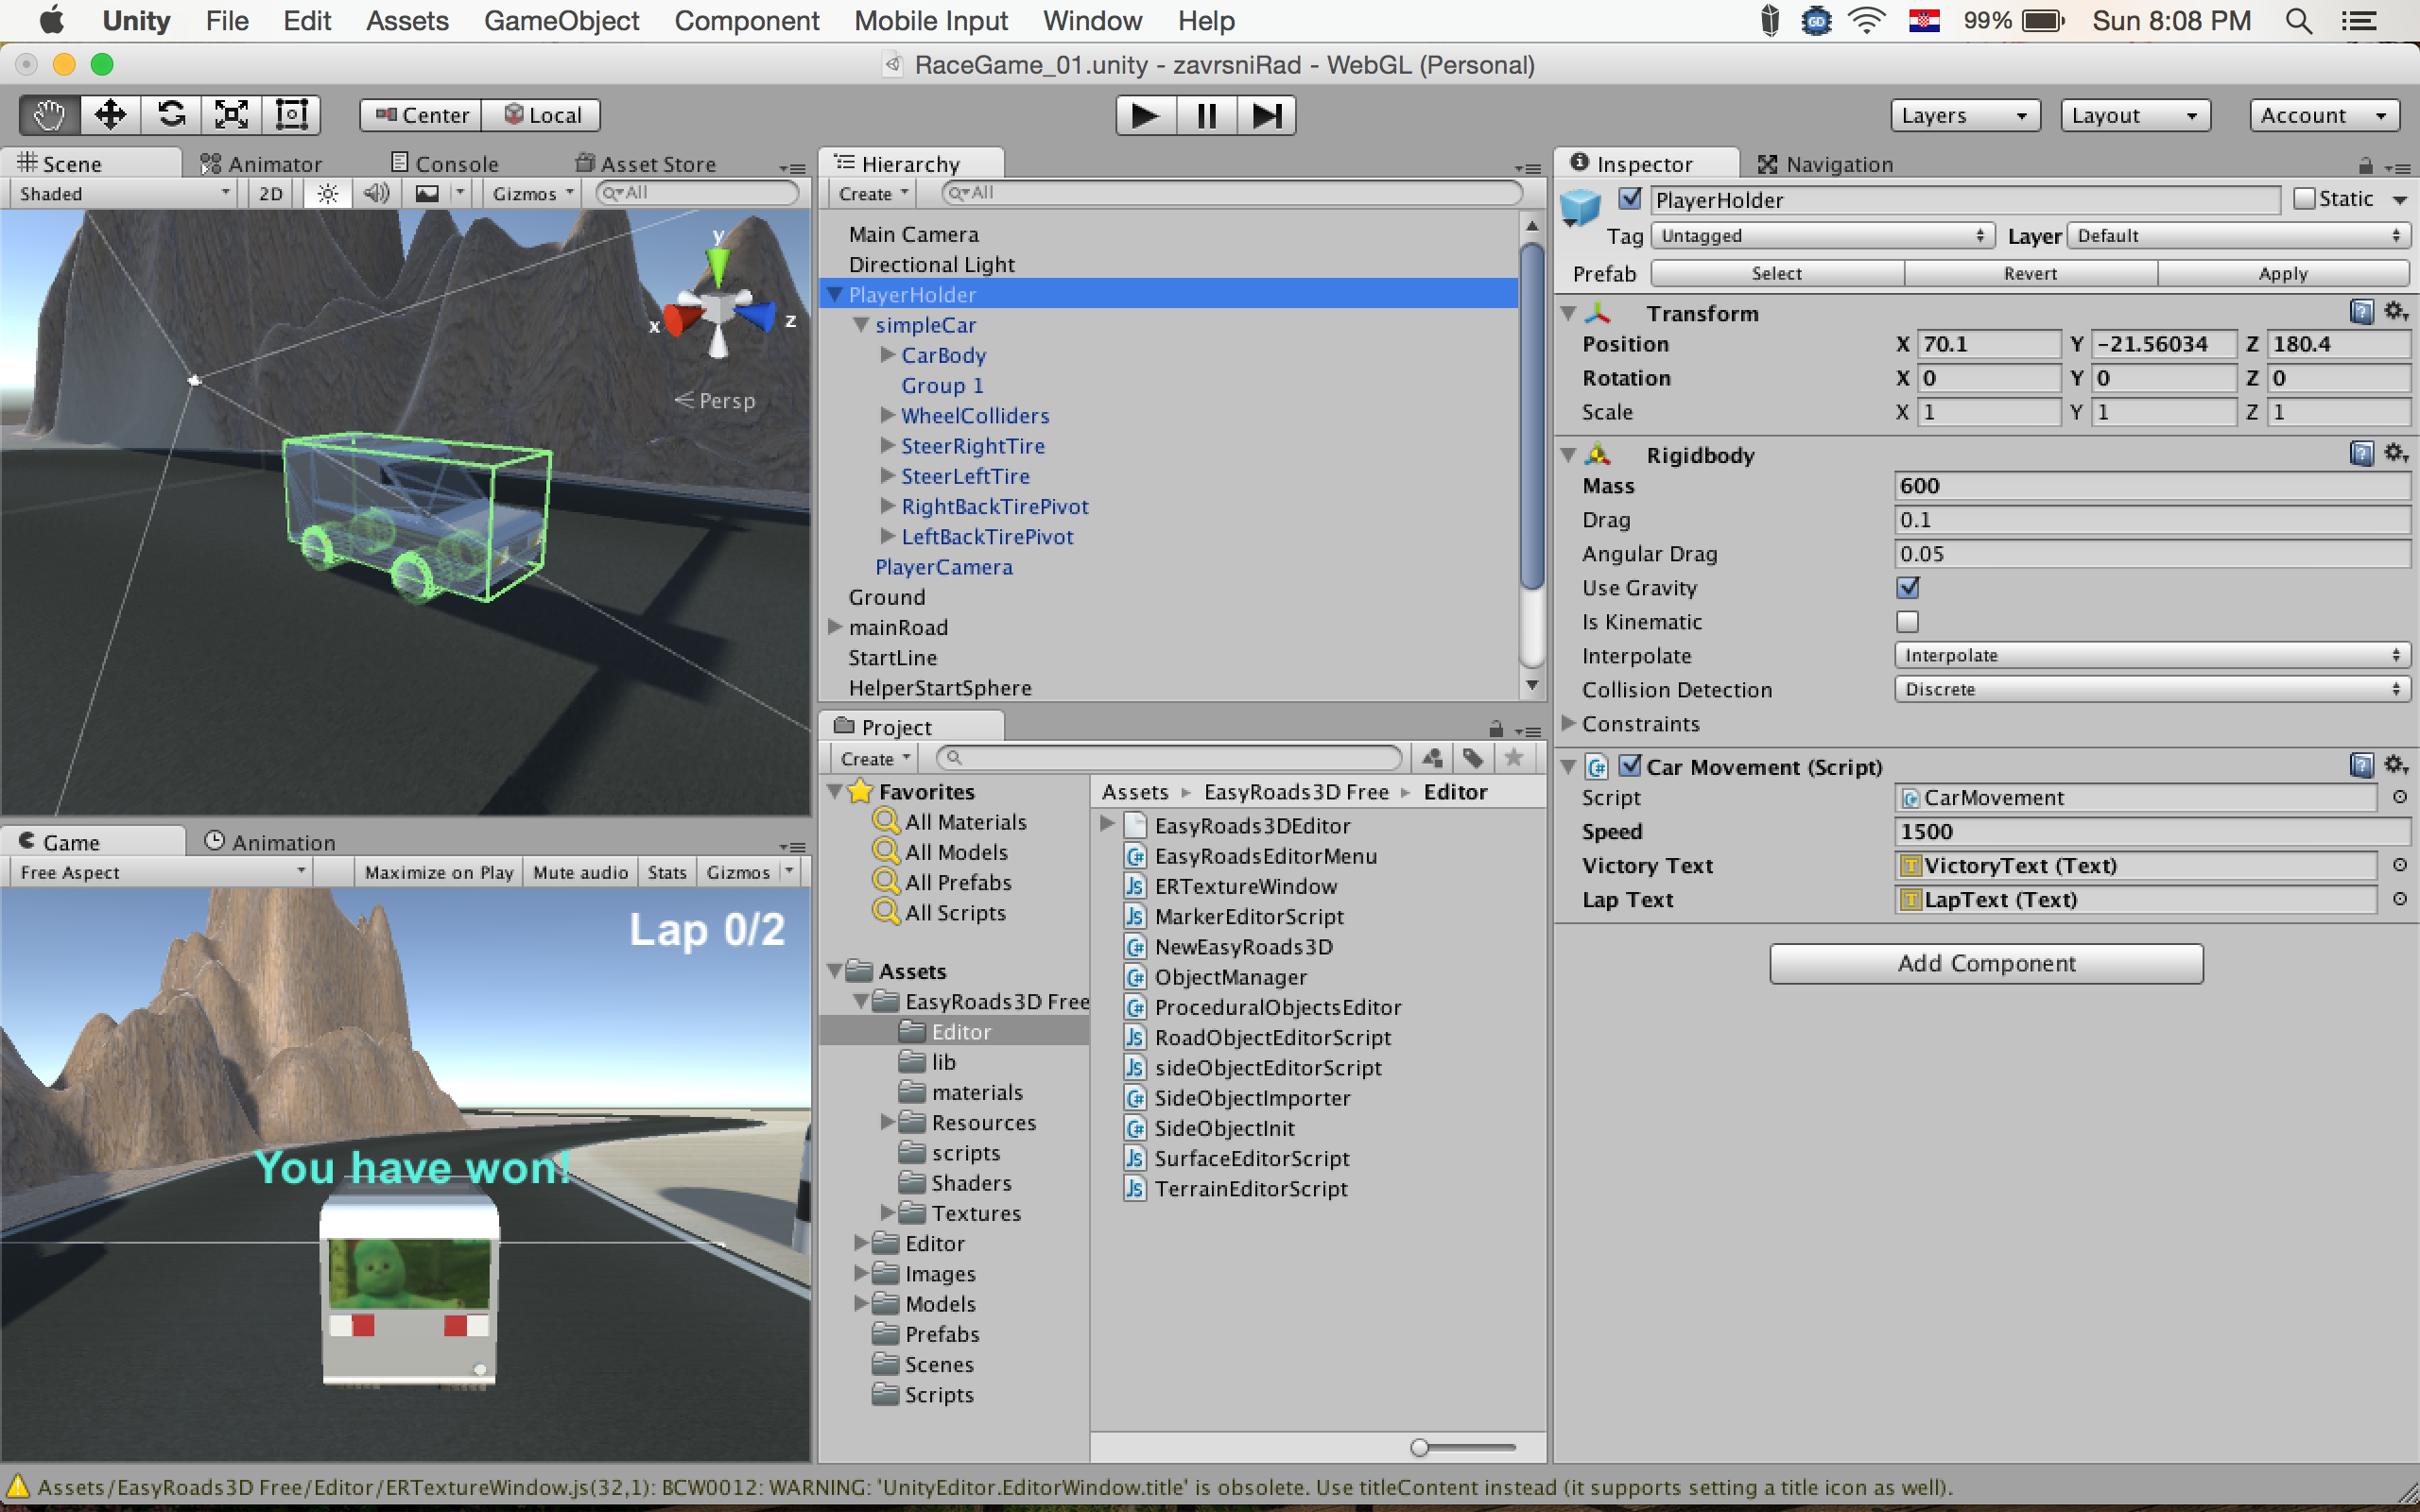
\includegraphics[width=12.5cm, height=10cm]{igrajuci_objekt.png}
	\centering
	\caption{Igrajući objekt}
	\label{fig:igrajuciobjekt}
\end{figure}
\newpage
Na slici broj \ref{fig:igrajuciobjekt} se može vidjeti primjer unity radne okoline i jedan igrajući objekt koji se zove "PlayerHolder". Ovaj igrajući objekt ima tri komponente, transformaciju, kruto tijelo i skriptu koja se zove "CarMovement". O skriptama i kako one funkcioniraju u sljedećem poglavlju. Dodavanje komponenti se može klikom na dugme "Add Component". Nakon klika na dugme se otvara padajući izbornik za odabir željene komponente. \par
Svaki igrajući objekt pripada jednom sloju (\emph{eng. Layer}) i ima oznaku (\emph{eng. Tag}). Kasnije se pomoću skripti može manipulirati ovim elementima provjerom njihovih slojeva i oznaka. U igri se korisei oznake upravo za provjeravanje, da li je korisnik prošao cestu pravim putem. Na slici broj \ref{fig:markeri} se mogu vidjeti markeri koji provjeravaju navedeno.
\subsection{Kamera}
Kamere se koriste za prikaz igre kako je programer zamislio. Koristeći više kamera moguće je napraviti različite efekte i animacije za igrača, te stvoriti jedinstveno iskustvo tijekom igranja igre. Kamere imaju dvije moguće projekcije (ortografijsku i perspektivnu). Ortografijska se koristi za 2D igrice ili ako nije bitna dubina u igricama. Najčešće su to neke platformske igre, puzzle ili slično. Perspektivna se koristi ako je želimo pokazati dubinu u igri. U igri se koristi ovaj oblik, te je postavljena kao dijete automobilskog igrajućeg objekta. Na ovaj način kamera slijedi automobil i dobiva se pravo iskustvo vožnje automobila.
\subsection{Svijetlo}
Svijetla se naravno koriste za osvijetljavanje svijeta, ali i za stvaranje ugođaja. Moguće je mijenjati boje svijetla, te tako stvarati prekrasne ambijente. Može se definirati spektar, doseg, boja, tip, intenzitet, intenzitet odbijanja, sjena i ostale naprednije funkcije. Zanimljivo je što se može definirati svijetlu da ne baca sjenu za igrajuće objekte. \par
Za bolju funkcionalnost se može preko padajućeg izbornika na svijetlu postaviti da je već ispečeno (\emph{eng. Baked}). Ovo znači da će se sva svijetla prilikom pokretanja igre izračunati i postaviti za igrajuće objekte koji se ne kreću. Ovo je veoma praktično jer nema potrebe preračunavati za te objekt njegov utjecaj sa svjetlom, već će se to obavljati ukoliko pokraj njega dođe ne-statičan objekt.
\subsection{Prefab}
Prefab je kao predložak za igrajuće objekte. Ako se koristi više istih igrajućih objekata, kao na primjer više istih automobila koji dijele sve funkcionalnosti. Tada nije praktično raditi promjene nad svakim automobilom zasebno, te se zato koriste prefabi. Kada se napravi novi igrajući objekt može se od njega napraviti prefab preko izbornika \emph{Asset}, pa zatim \emph{Create Prefab}. Nakon što se napravi prefab može se jednostavno povlačiti u svijet, te tako stvarati nove instance igrajućih objekata, koje dijele iste funkcionalnosti. Sada ako se nešto želi promijeniti, može se mijenjati bilo koji od objekata i unity će pitati, da li treba obaviti ove promjene i na ostale instance ovog prefaba.